\section{Inpainting}

In dit hoofdstuk zullen we wavelets gebruiken om ontbrekende regio's in foto's in te kleuren. Deze methode wordt gebruikt om beschadigde foto's te reconstrueren. De schade op de foto wordt gemodelleerd met pixel waarden in de foto die verdwenen zijn. Om de verdwenen regio's in te kleuren wordt de iteratieve methode gebruikt die beschreven staat in de opgave. We hebben dit algoritme ge\"{i}mplementeerd in Matlab met behulp van de Wavelet toolbox. Hierbij nemen we een bepaalde foto en verwijderen we de pixels in bepaalde regio's. Het algoritme probeert dan de verdwenen regio's in te kleuren. 
\newline
\newline
In figuur \ref{fig:matti_fig_1} wordt het algoritme ge\"{i}llustreerd met verschillende soorten regio's van pixels die verwijderd zijn. In figure \ref{fig:matti_fig_1a} zijn er blokken pixels verwijderd, in figuur \ref{fig:matti_fig_1c} zijn er random pixels verwijderd en in figuur \ref{fig:matti_fig_1e} is de figuur overschreven met tekst. De resultaten van het 'inpainting' algoritme staan er steeds naast. Het algoritme geeft op het eerste zicht heel mooie resultaten. Alleen als we de ingekleurde resultaten in detail gaan bekijken merken we dat het niet de originele figuren zijn. Dit is het meest duidelijk bij de figuren die bewerkt zijn met blokken en met tekst.


\begin{figure}
    \centering
    \begin{subfigure}[b]{0.45\textwidth}
        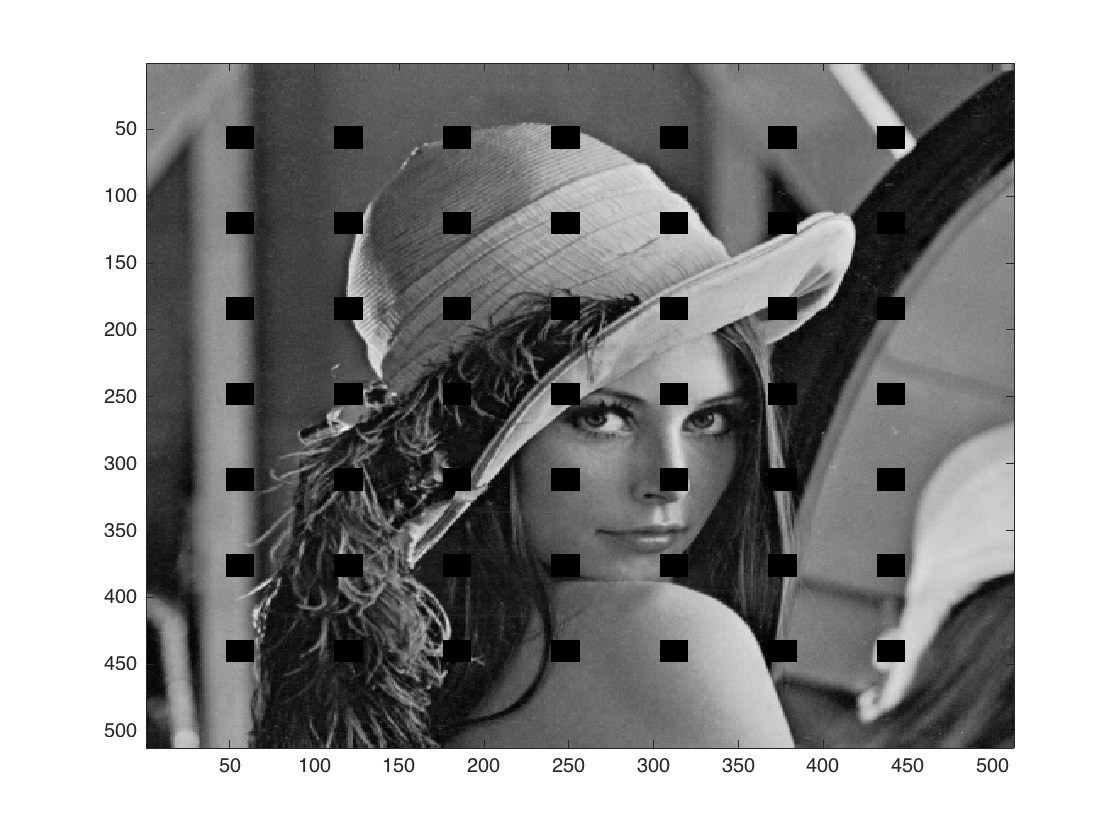
\includegraphics[width=\textwidth]{../src/inpainting/lena_block}
        \caption{Foto van Lena met vierkante blokjes pixels verwijderd (zwart gemaakt). }
        \label{fig:matti_fig_1a}
    \end{subfigure}
    ~ %add desired spacing between images, e. g. ~, \quad, \qquad, \hfill etc. 
    %(or a blank line to force the subfigure onto a new line)
    \begin{subfigure}[b]{0.45\textwidth}
        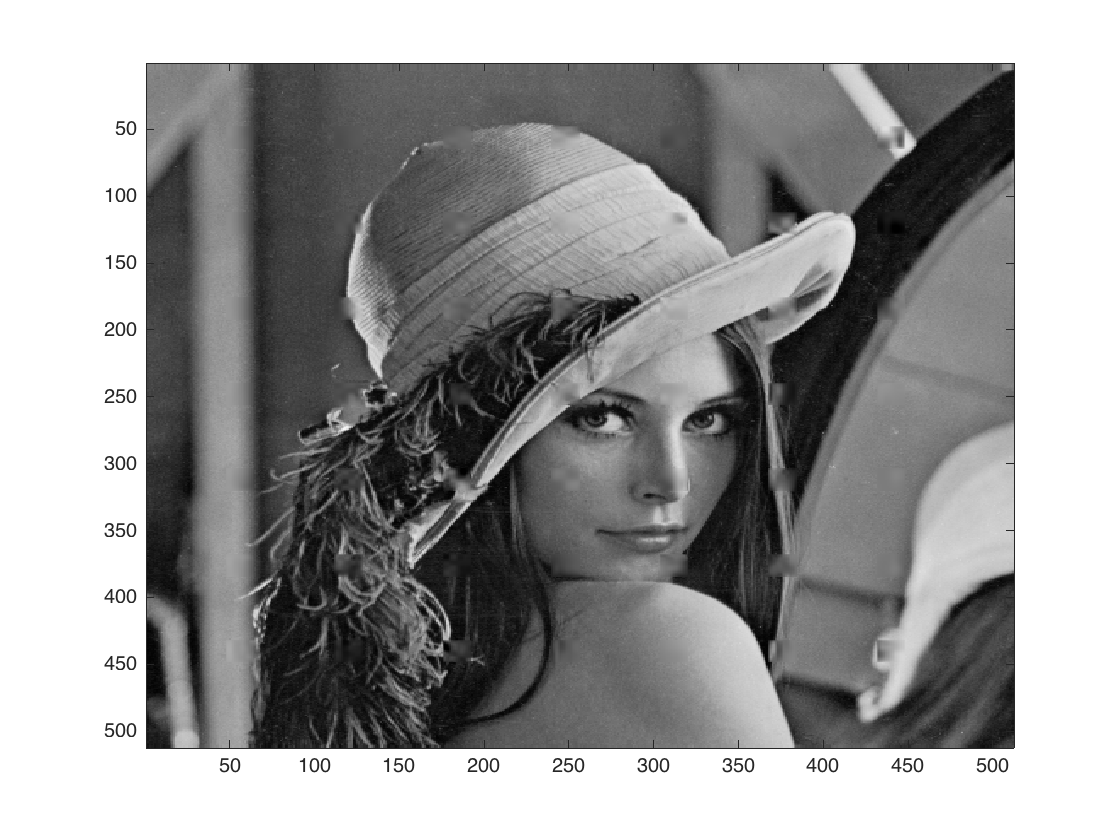
\includegraphics[width=\textwidth]{../src/inpainting/lena_blok_painted_1}
        \caption{Foto \ref{fig:matti_fig_1a} ingekleurd. \\ \ \\}
        \label{fig:matti_fig_1b}
    \end{subfigure}
    \begin{subfigure}[b]{0.45\textwidth}
        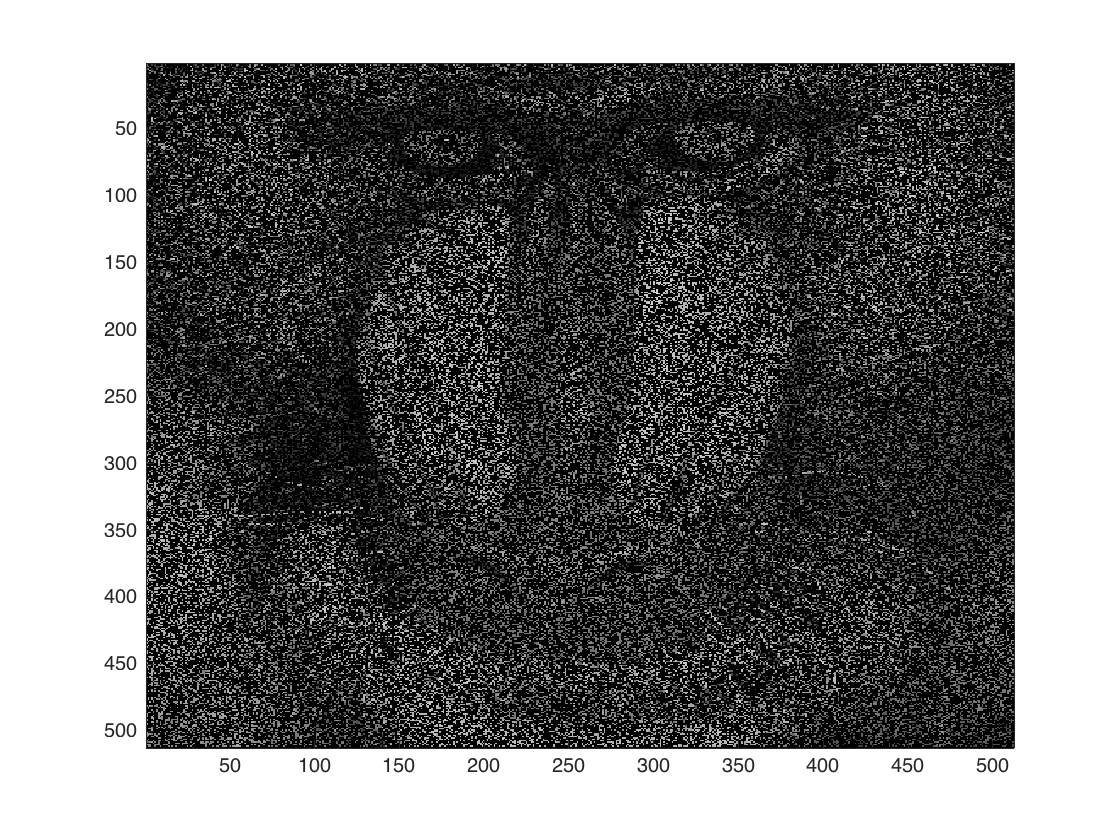
\includegraphics[width=\textwidth]{../src/inpainting/baboon_random_noise_1}
        \caption{Foto van aap met ongeveer 70 procent van de pixels verwijderd (zwart gemaakt). }
        \label{fig:matti_fig_1c}
    \end{subfigure}
    ~ %add desired spacing between images, e. g. ~, \quad, \qquad, \hfill etc. 
    %(or a blank line to force the subfigure onto a new line)
    \begin{subfigure}[b]{0.45\textwidth}
        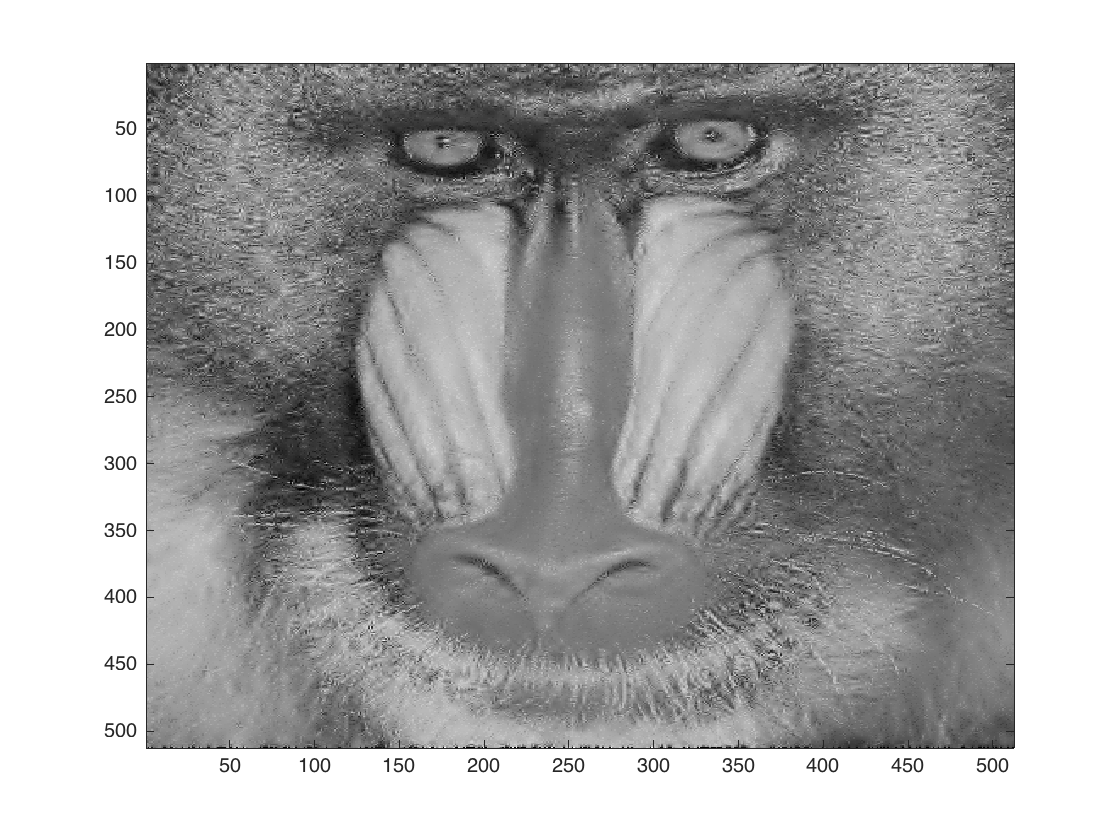
\includegraphics[width=\textwidth]{../src/inpainting/baboon_random_fixed_1}
        \caption{Foto \ref{fig:matti_fig_1c} ingekleurd. \\ \ \\}
        \label{fig:matti_fig_1d}
    \end{subfigure}
        \begin{subfigure}[b]{0.45\textwidth}
        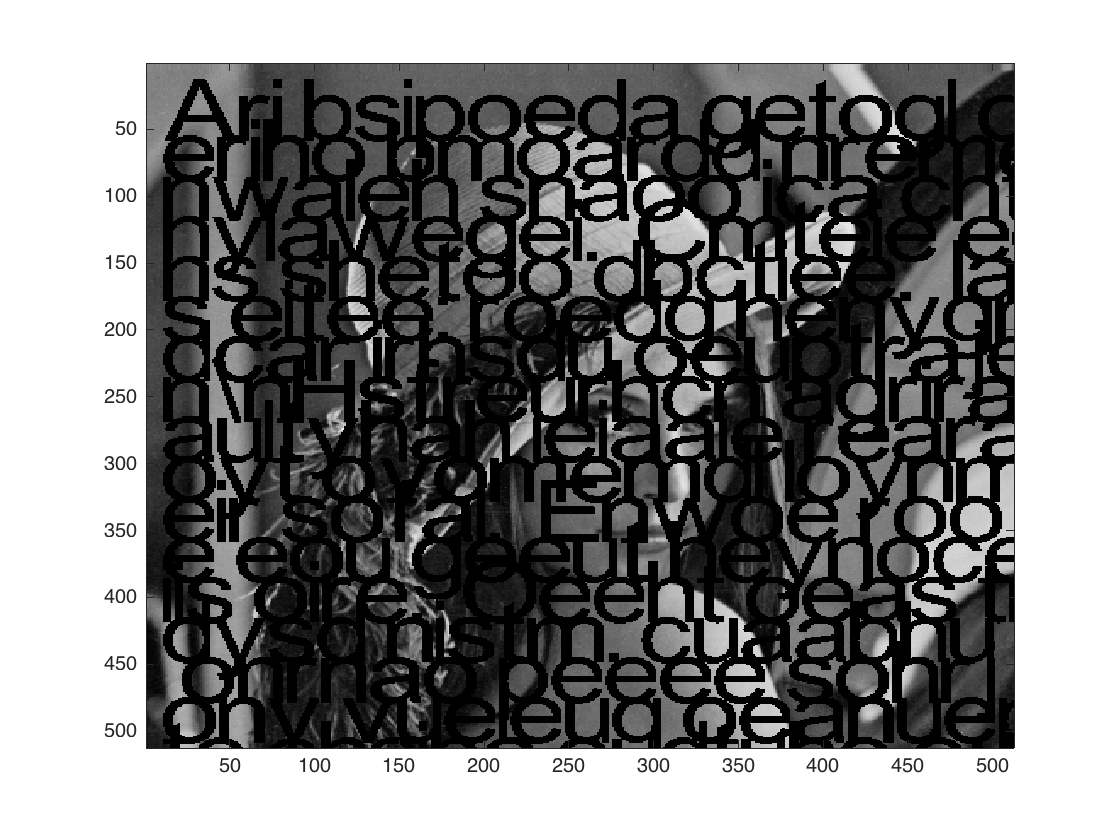
\includegraphics[width=\textwidth]{../src/inpainting/lena_letters_broke_1}
        \caption{Foto van lena overschreven met tekst. }
        \label{fig:matti_fig_1e}
    \end{subfigure}
    ~ %add desired spacing between images, e. g. ~, \quad, \qquad, \hfill etc. 
    %(or a blank line to force the subfigure onto a new line)
    \begin{subfigure}[b]{0.45\textwidth}
        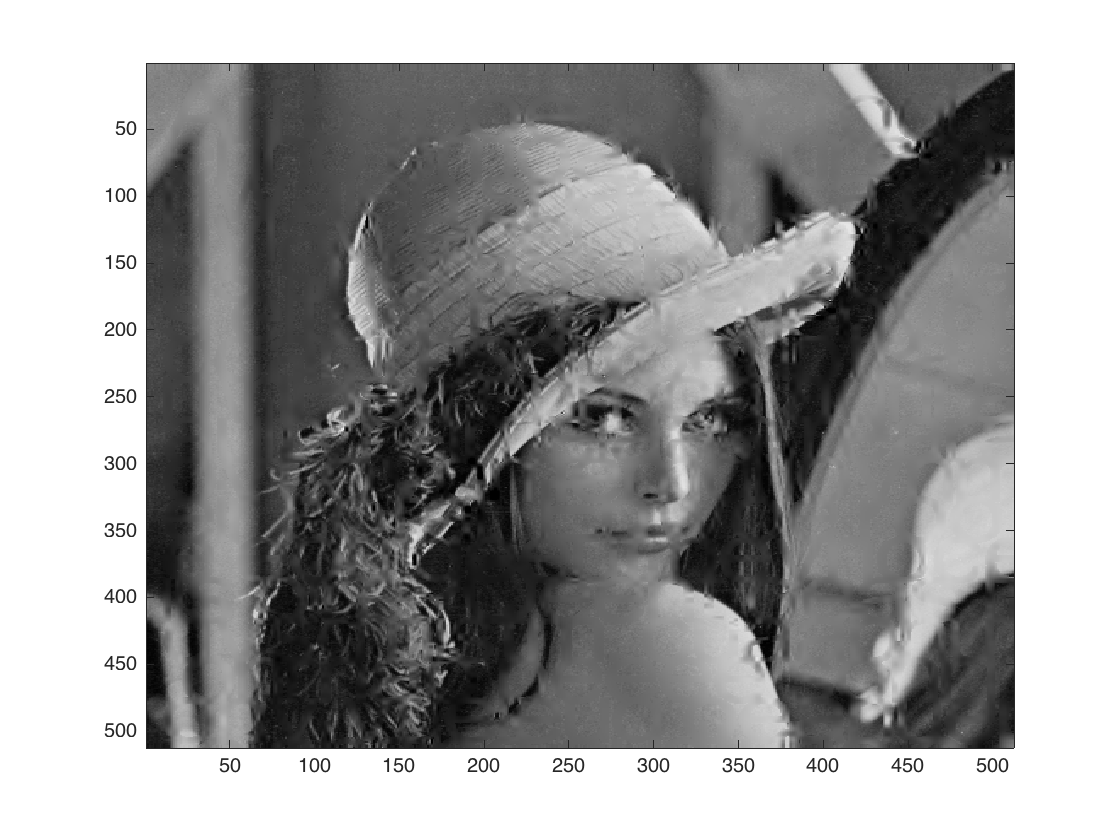
\includegraphics[width=\textwidth]{../src/inpainting/lena_letters_fixed_1}
        \caption{Foto \ref{fig:matti_fig_1e} ingekleurd.}
        \label{fig:matti_fig_1f}
    \end{subfigure}
    \caption{Resultaten van het 'Inpainting' algoritme. Instellingen algoritme: wavelet: 'db5', level $N = 10$, soft thresholding, threshold parameter $\delta = 10$, 200 iteraties.}\label{fig:matti_fig_1}
\end{figure}

%\FloatBarrier

Het 'inpainting' algoritme kan gebruikt worden op verschillende manieren. Zo zijn er verschillende soorten wavelets die gebruikt kunnen worden. De thresholding kan op verschillende manieren gebeuren en de threshold parameter $\delta$ moet gekozen worden. De effecten op het resultaat van al deze verschillende soorten instellingen zullen besproken worden in de volgende hoofdstukken.

%\FloatBarrier


\subsection{Threshold technieken}

\begin{figure}[!]
    \centering
    \begin{subfigure}[b]{0.45\textwidth}
        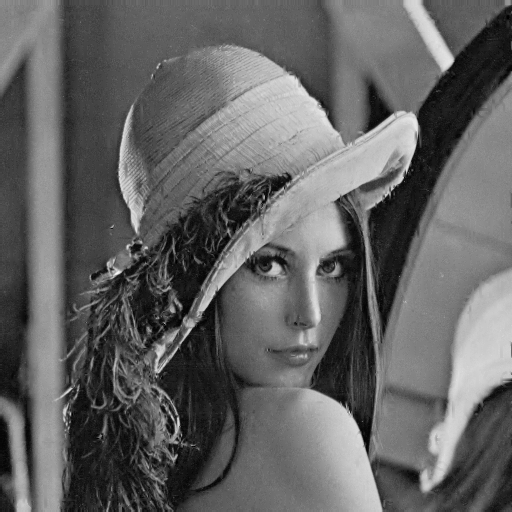
\includegraphics[width=\textwidth]{../src/inpainting/lena_soft_2}
        \caption{ \textbf{Soft thresholding ($\mathbf{\delta = 10 }$)}.}
        \label{fig:matti_soft_2}
    \end{subfigure}
    ~ %add desired spacing between images, e. g. ~, \quad, \qquad, \hfill etc. 
    %(or a blank line to force the subfigure onto a new line)
    \begin{subfigure}[b]{0.45\textwidth}
        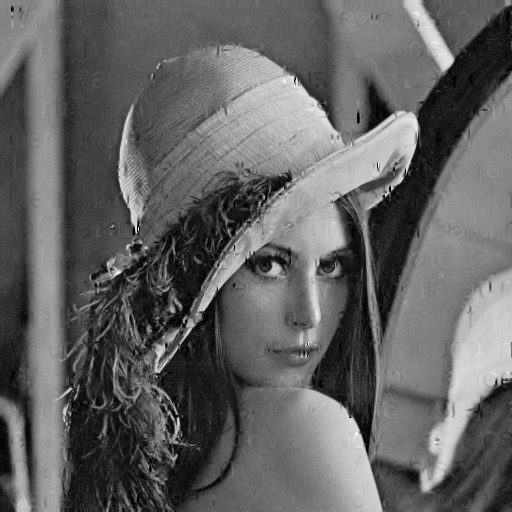
\includegraphics[width=\textwidth]{../src/inpainting/lena_hard_2}
        \caption{ \textbf{Hard thresholding ($\mathbf{\delta = 100 }$)}.}
        \label{fig:matti_hard_2}
    \end{subfigure}
    \caption{Met tekst overschreven figuur \ref{fig:matti_fig_1e} ingekleurd met 'inpainting' algoritme. Instellingen algoritme: wavelet: 'db5', level $N = 10$, 200 iteraties.}\label{fig:matti_hardsoft}
\end{figure}

%\FloatBarrier


Er zijn 2 soorten technieken voor thresholding, namelijk soft thresholding en hard thresholding. Voor beide technieken moet ook een threshold parameter $\delta > 0$ gekozen worden. In figuur \ref{fig:matti_hardsoft} is een figuur ingekleurd op twee manieren. E\'{e}n keer met soft thresholding en threshold parameter $\delta = 10$ en de andere keer met hard thresholding en threshold parameter $\delta = 100$. In het geval van soft thresholding was het gemakkelijk om een threshold parameter te vinden die redelijk goede resultaten geeft. Voor hard thresholding was het langer zoeken achter een geschikte threshold parameter $\delta = 100$. Dit was de meest optimale waarde van $\delta$ die ik op het eerste zicht kon vinden. Het is duidelijk dat voor soft thresholding betere resultaten kunnen bekomen worden als voor hard thresholding. Bij hard thresholding zijn er nog veel randen van letters zichtbaar. Bij soft thresholding zijn de resultaten veel beter. 
\newline
\newline
Het is duidelijk dat het vinden van de optimale threshold parameter $\delta$ niet zo eenvoudig is. Daarom zullen we het volgende experiment uitvoeren. We voeren het 'inpainting' algoritme uit voor een reeks van verschillende waardes van $\delta$. Voor elke waarde van $\delta$ zal het relatieve verschil tussen de ingekleurde foto en de originele onbeschadigde foto berekent worden. Dit verschil wordt voorgesteld op de volgende manier:

\begin{equation} \label{eq:matti_eq1}
\frac{\left\lVert A_{\text{ingekleurd}} - A_{\text{onbeschadigd}} \right\rVert_{F}}{\left\lVert A_{\text{onbeschadigd}} \right\rVert_{F}}
\end{equation}

\begin{figure}
  \centering
    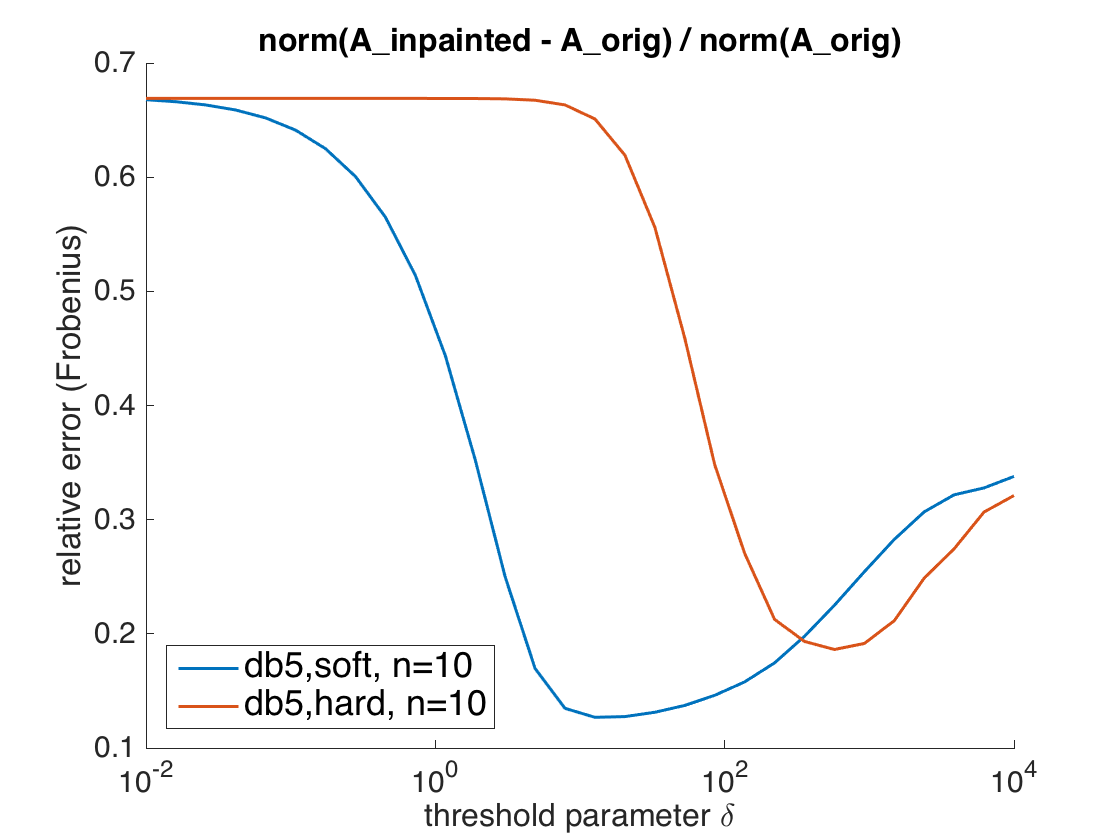
\includegraphics[width=0.8\textwidth]{../src/inpainting/error_plot_3}
    \caption{Het relatieve verschil beschreven \eqref{eq:matti_eq1} in functie van de threshold parameter $\delta$ voor zowel soft als hard thresholding. Instellingen algoritme: wavelet: 'db5', level $N = 10$, 50 iteraties voor elke waarde van $\delta$. Het relatieve verschil tussen de onbeschadigde en de beschadige foto is ongeveer $0.67$. De foto van lena overschreven met tekst van in figuur \ref{fig:matti_fig_1e} is gebruikt.}
    \label{fig:matti_error_plot_3}
\end{figure}

\begin{figure}
    \centering
    \begin{subfigure}[b]{0.45\textwidth}
        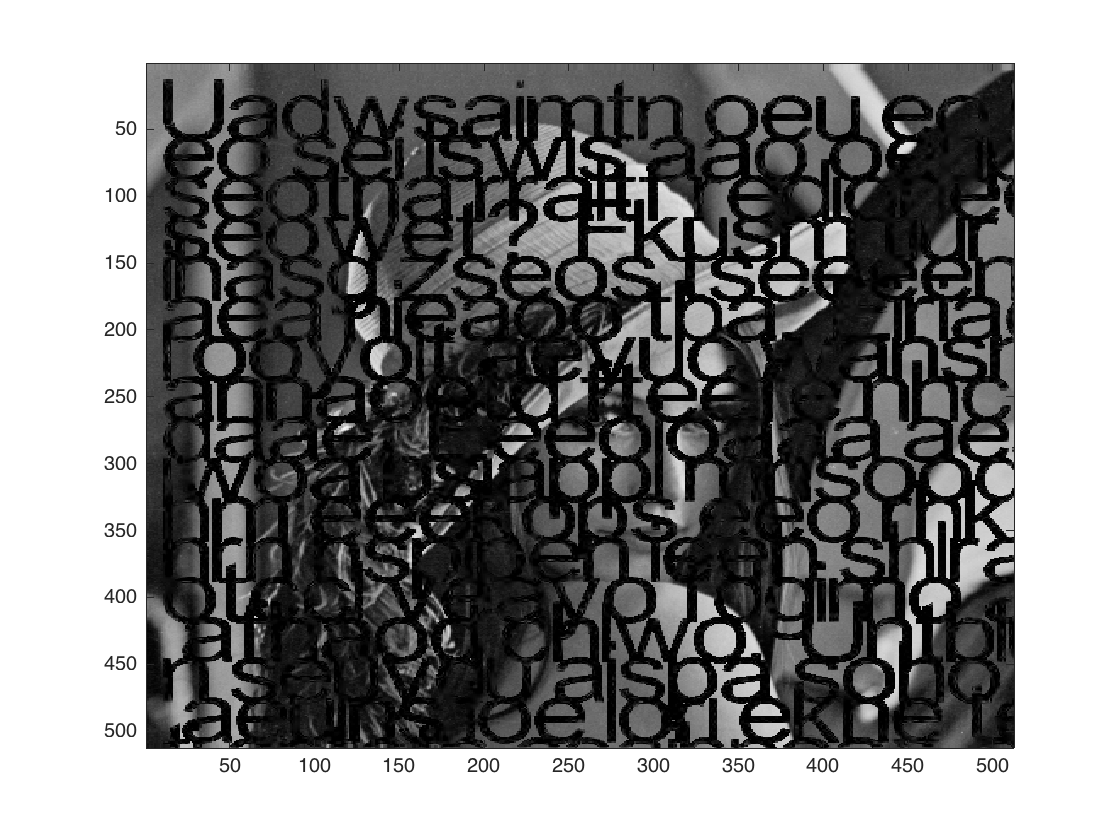
\includegraphics[width=\textwidth]{../src/inpainting/lena_failed_4}
        \caption{ \textbf{Hard thresholding} met te lage waarde van $\mathbf{\delta = 10 }$ . (volgens figuur \ref{fig:matti_error_plot_3})}
        \label{fig:matti_failed_4}
    \end{subfigure}
    ~ %add desired spacing between images, e. g. ~, \quad, \qquad, \hfill etc. 
    %(or a blank line to force the subfigure onto a new line)
    \begin{subfigure}[b]{0.45\textwidth}
        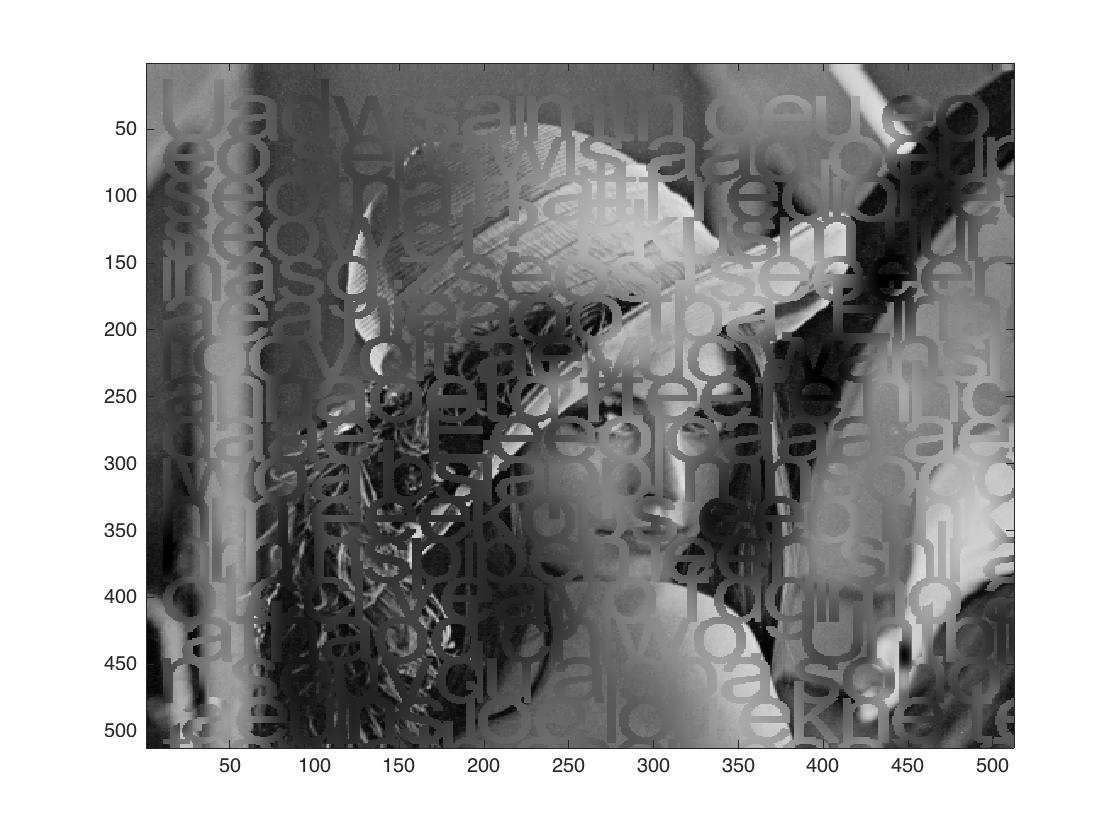
\includegraphics[width=\textwidth]{../src/inpainting/lena_optimal_4}
        \caption{\textbf{Hard thresholding} met de optimale waarde van $\mathbf{\delta = 1000 }$ . (volgens figuur \ref{fig:matti_error_plot_3})}
        \label{fig:matti_optimal_4}
    \end{subfigure}
    \caption{Met tekst overschreven figuur \ref{fig:matti_fig_1e} ingekleurd met 'inpainting' algoritme. Instellingen algoritme: wavelet: 'db5', level $N = 10$, hard thresholding, 200 iteraties. De inkleuring in de linkse figuur is volleding mislukt vanwege een blijkbaar te lage waarde van $\delta$.} \label{fig:matti_hard_4}
\end{figure}

met $A$ de matrix met pixel waarden corresponderend met de foto. In figuur \ref{fig:matti_error_plot_3} kan men duidelijk het verschil zien tussen soft en hard thresholding. Soft thresholding bereikt een lager minimum rond de optimale waarde $\delta = 10$. Het minimum bij hard thresholding ligt iets hoger en wordt bereikt voor veel grotere waarden van $\delta$. Opmerkelijk is dat hard thresholding het heel slecht doet indien de parameter $\delta$ relatief klein in tegenstelling tot soft thresholding. In figuur \ref{fig:matti_hard_4} is hard thresholding gebruikt met een te lage waarde van $\delta$ en de optimale waarde van $\delta$ (minimum rode curve figuur \ref{fig:matti_error_plot_3}). Met $\delta = 10$ mislukt het inkleuren volledig. Dit was te verwachten als we kijken naar figuur \ref{fig:matti_error_plot_3}. Volgens figuur \ref{fig:matti_error_plot_3} zou de optimale waarde van $\delta$ bij hard thresholding rond $1000$ moeten liggen. Hoewel figuur \ref{fig:matti_optimal_4} ($\delta = 1000$)  niet heel slecht is, verkies ik persoonlijk toch figuur \ref{fig:matti_hard_2} ($\delta = 100$) boven figuur \ref{fig:matti_optimal_4} alhoewel het relatieve verschil voor resultaat \ref{fig:matti_optimal_4} minder is. In figuur \ref{fig:matti_optimal_4} zijn nog heel duidelijk de letters te zien. De conclusie is dus dat men niet louter naar het minimale verschil in norm moet kijken maar ook naar het bekomen resultaat. Een tweede conclusie is dat soft thresholding het veel beter doet als hard thresholding voor meer verschillende ordes van $\delta$. Soft thresholding heeft minder last met de randen van de letters in tegenstelling tot hard thresholding.



\subsection{Redundant vs non-redundant wavelet transformaties}

In dit hoofdstuk zullen we kort het verschil bestuderen tussen redundant en non-redundant wavelet transformaties. In figuur \ref{fig:matti_fig_rwt} zijn 6 ingekleurde figuren getoond. Hierbij zijn 3 soorten wavelets gebruikt en voor elke soort wavelet is de non-redundant en redundant wavelet transformatie uitgetest. Bij elke figuur is de corresponderende SNR waarde getoond. Het is duidelijk dat de bekomen resultaten veel beter zijn bij de redundant wavelet transformaties. Dit is zowel te zien in de figuren als in de SNR waardes. De 'overbodige' informatie dat de redundant wavelet transformatie gebruikt is blijkbaar toch niet zo overbodig in het geval van 'inpainting' toepassingen. Opmerkelijk is dat voor de biorthogonale spline wavelet gebruikt in figuur \ref{fig:matti_fig_rwt} het resultaat volledig mislukt is voor de non-redundant wavelet transformatie en voor de redundant wavelet transformatie het resultaat juist heel goed is. Dit is te zien in figuur \ref{fig:matti_fig_wt_bior33} en figuur \ref{fig:matti_fig_rwt_bior33}.
\newline
\newline
Het enigste nadeel bij redundant wavelet transformaties is dat de rekentijd bij wavelet transformaties een stuk hoger ligt. Deze rekentijd bij redundant wavelet transformaties stijgt ook veel bij hoger gebruikte levels in de transformatie. In ons geval kon het iteratieproces in het 'inpainting' algoritme gemakkelijk 10 keer zoveel rekentijd vragen voor de redundant wavelet transformaties in vergelijking met de non-redundant wavelet transformaties.

\subsection{Wavelet soorten}

In dit hoofdstuk zal kort het verschil in de resultaten tussen verschillende type wavelets besproken worden. In figuur \ref{fig:matti_fig_5} zijn de 'inpainting' resultaten getoond voor 6 verschillende soorten wavelets. De SNR waarden zijn er steeds bij vermeld. In figuur \ref{fig:matti_fig_haar} is de Haar wavelet gebruikt. In deze figuur zijn kleine blokjes te zien, Dit is omdat de Haar wavelet niet geschikt is voor continue overgangen. De corresponderende SNR waarde is $16.19$. De 2 Daubechies wavelets in figuur \ref{fig:matti_fig_db2} en \ref{fig:matti_fig_db6} doen het beter als de haar wavelet. Dit is zowel te zien in de figuur als de SNR waarde. De reden hiervoor is dat Daubechies wavelets beter geschikt zijn voor continue overgangen. In figuur \ref{fig:matti_fig_bior33} is een biorthogonale spline wavelet gebruikt. In deze figuur is een heel slecht resultaat bekomen. De beste resultaten zijn bij de Coiflet en Symlet wavelet in figuur \ref{fig:matti_fig_coif4} en figuur \ref{fig:matti_fig_sym5}.

\begin{figure}
    \centering
    \begin{subfigure}[b]{0.45\textwidth}
        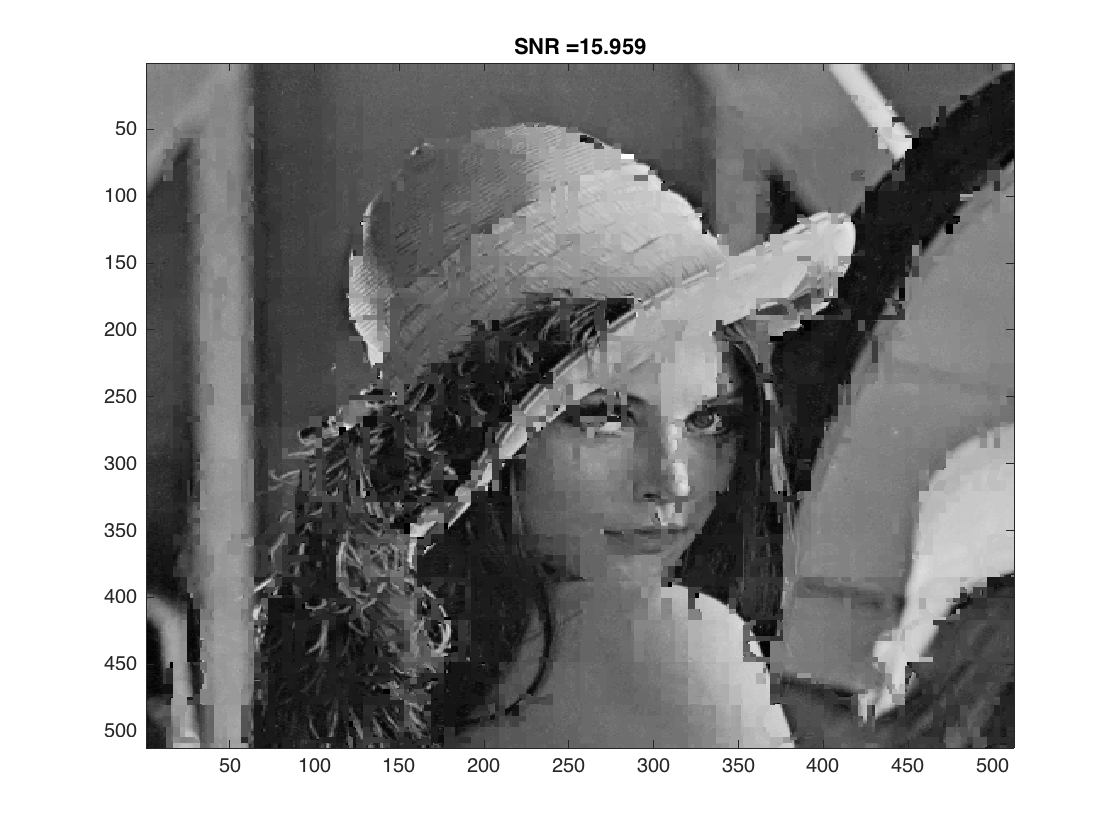
\includegraphics[width=\textwidth]{../src/inpainting/vraag_2_3_wt_haar}
        \caption{\textbf{Non-redundant Haar wavelet, \\ SNR = $\mathbf{15.96}$} }
        \label{fig:matti_fig_wt_haar}
    \end{subfigure}
    ~ %add desired spacing between images, e. g. ~, \quad, \qquad, \hfill etc. 
    %(or a blank line to force the subfigure onto a new line)
    \begin{subfigure}[b]{0.45\textwidth}
        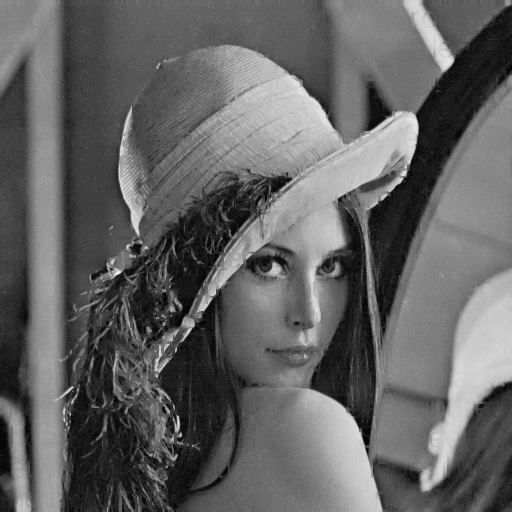
\includegraphics[width=\textwidth]{../src/inpainting/vraag_2_3_rwt_haar}
        \caption{\textbf{Redundant Haar wavelet, \\ SNR = $\mathbf{18.15}$} }
        \label{fig:matti_fig_rwt_haar}
    \end{subfigure}
    \begin{subfigure}[b]{0.45\textwidth}
        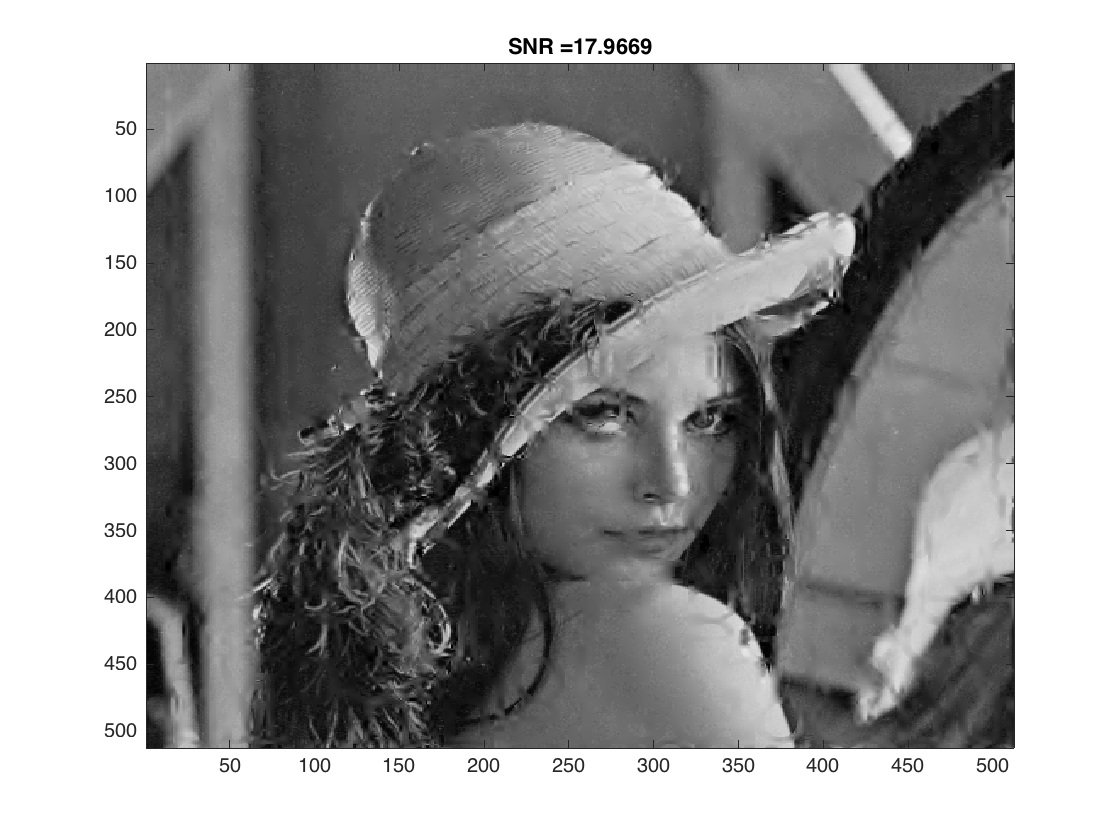
\includegraphics[width=\textwidth]{../src/inpainting/vraag_2_3_wt_db5}
        \caption{\textbf{Non-redundant Daubechies (db5) wavelet,  SNR = $\mathbf{17.97}$} }
        \label{fig:matti_fig_wt_db5}
    \end{subfigure}
    ~ %add desired spacing between images, e. g. ~, \quad, \qquad, \hfill etc. 
    %(or a blank line to force the subfigure onto a new line)
    \begin{subfigure}[b]{0.45\textwidth}
        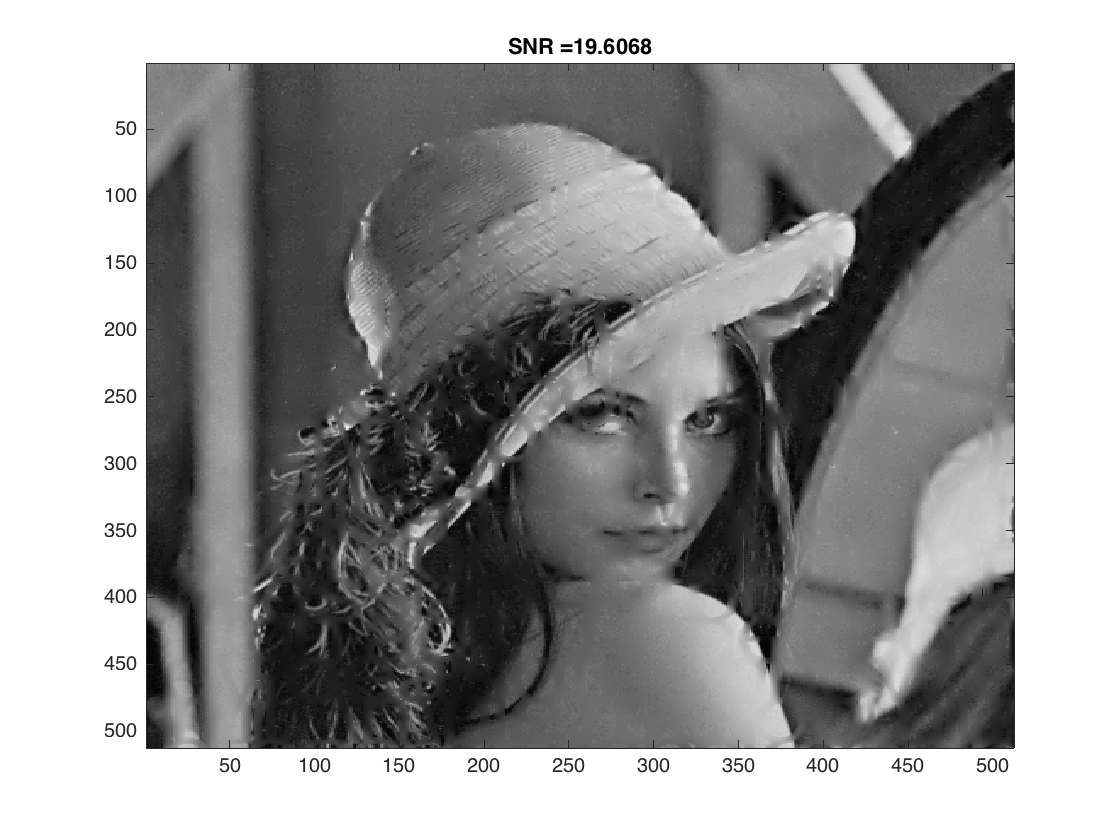
\includegraphics[width=\textwidth]{../src/inpainting/vraag_2_3_rwt_db5}
        \caption{\textbf{ Redundant Daubechies (db5) wavelet, SNR = $\mathbf{19.61}$} }
        \label{fig:matti_fig_rwt_db5}
    \end{subfigure}
        \begin{subfigure}[b]{0.45\textwidth}
        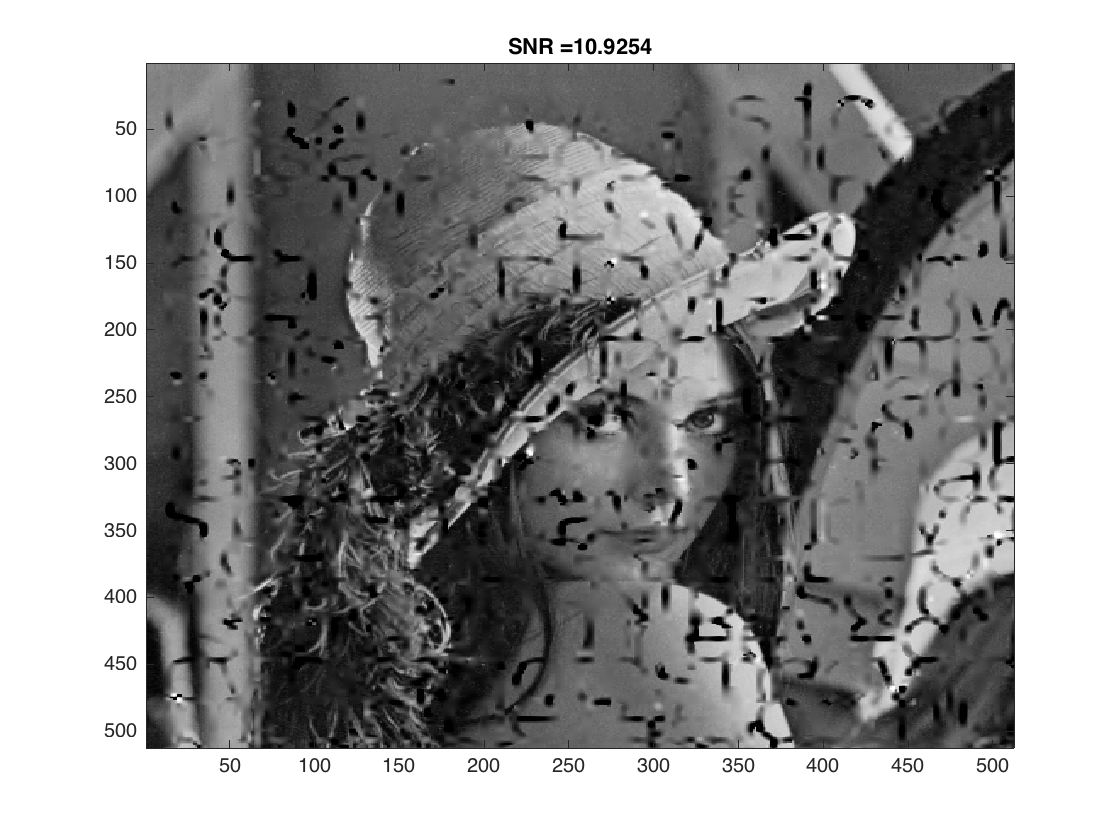
\includegraphics[width=\textwidth]{../src/inpainting/vraag_2_3_wt_bior33}
        \caption{\textbf{ Non-redundant CDF (bior3.3) wavelet, SNR = $\mathbf{10.93}$} }
        \label{fig:matti_fig_wt_bior33}
    \end{subfigure}
    ~ %add desired spacing between images, e. g. ~, \quad, \qquad, \hfill etc. 
    %(or a blank line to force the subfigure onto a new line)
    \begin{subfigure}[b]{0.45\textwidth}
        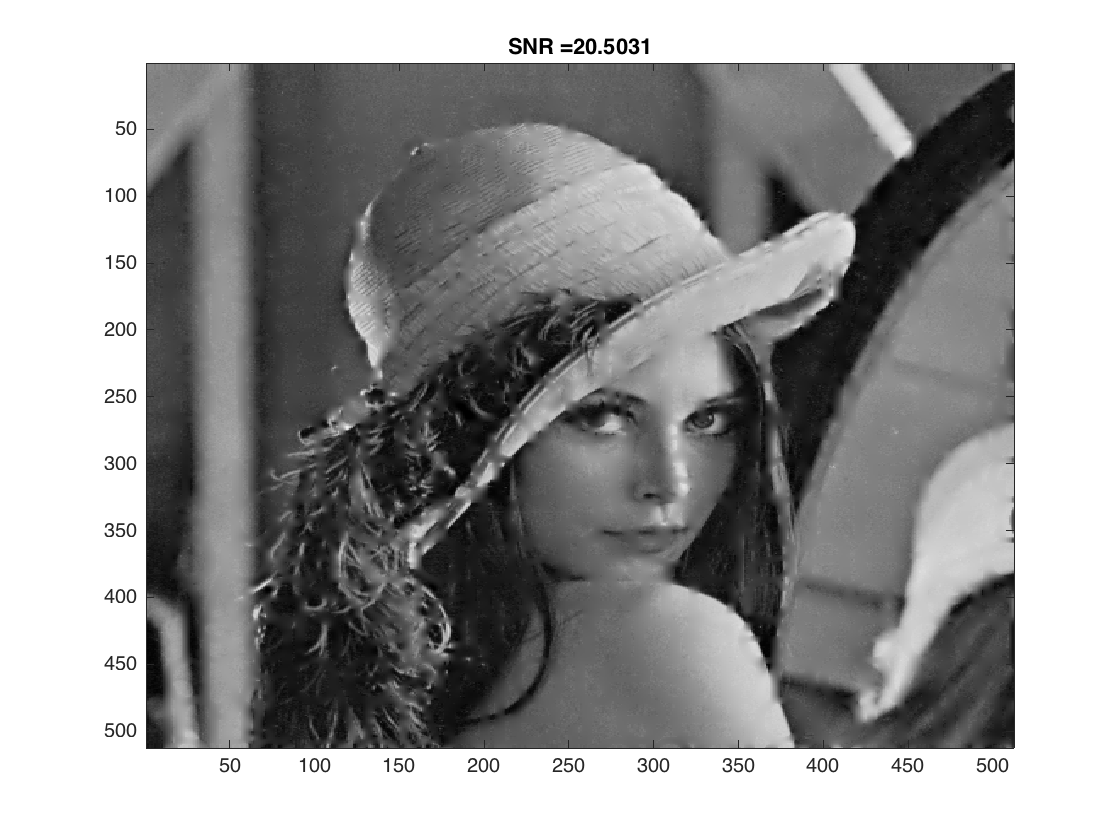
\includegraphics[width=\textwidth]{../src/inpainting/vraag_2_3_rwt_bior33}
        \caption{\textbf{ Redundant CDF (bior3.3) wavelet, SNR = $\mathbf{20.50}$} }
        \label{fig:matti_fig_rwt_bior33}
    \end{subfigure}
    \caption{Resultaten van het 'Inpainting' algoritme voor verschillende soorten wavelets. Instellingen algoritme: level $N = 6$, soft thresholding, threshold parameter $\delta = 10$, 200 iteraties.}\label{fig:matti_fig_rwt}
\end{figure}


\begin{figure}
    \centering
    \begin{subfigure}[b]{0.45\textwidth}
        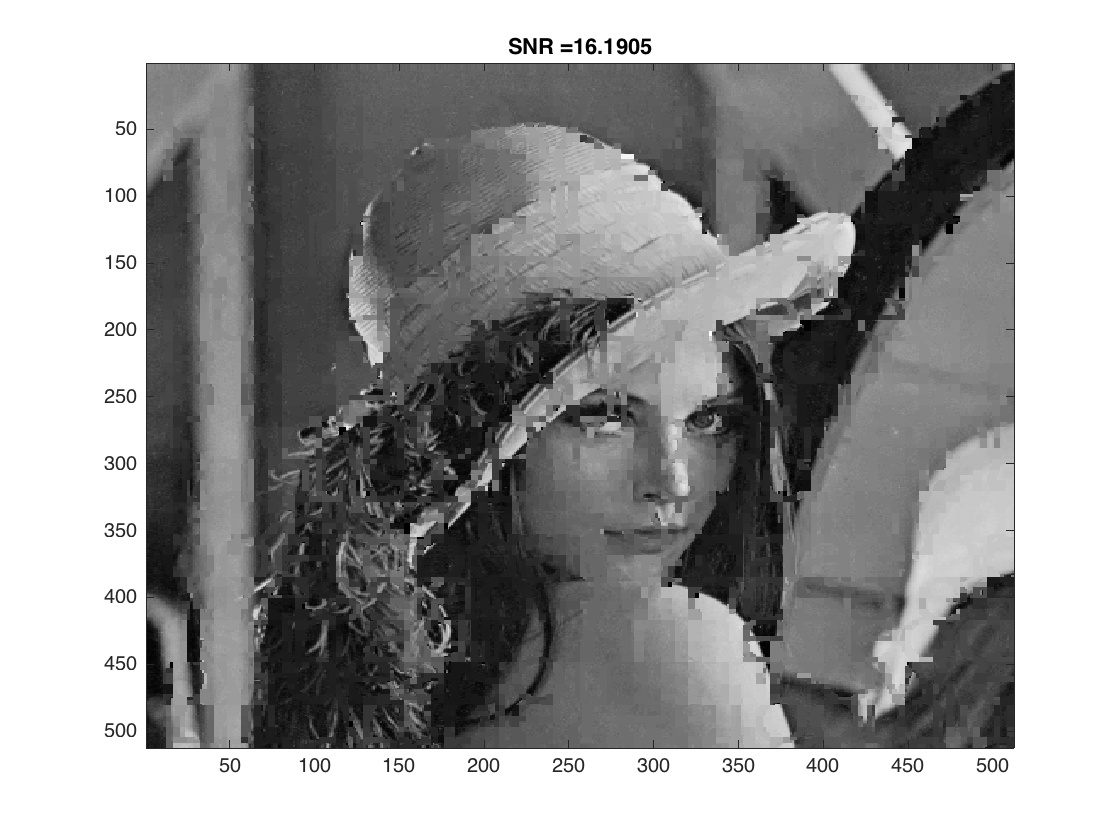
\includegraphics[width=\textwidth]{../src/inpainting/vraag_2_4_haar}
        \caption{\textbf{Haar wavelet, \\ SNR = $\mathbf{16.19}$} }
        \label{fig:matti_fig_haar}
    \end{subfigure}
    ~ %add desired spacing between images, e. g. ~, \quad, \qquad, \hfill etc. 
    %(or a blank line to force the subfigure onto a new line)
    \begin{subfigure}[b]{0.45\textwidth}
        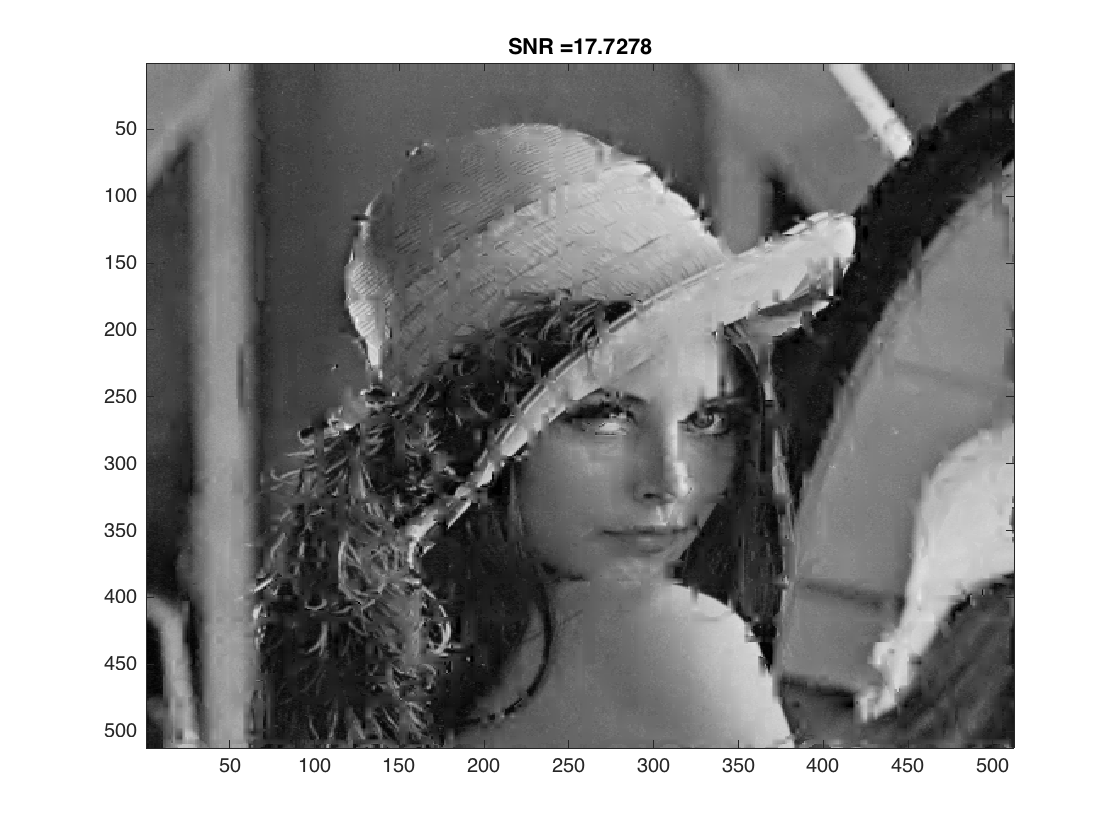
\includegraphics[width=\textwidth]{../src/inpainting/vraag_2_4_db2}
        \caption{\textbf{Daubechies 'db2' wavelet, \\ SNR = $\mathbf{17.73}$} }
        \label{fig:matti_fig_db2}
    \end{subfigure}
    \begin{subfigure}[b]{0.45\textwidth}
        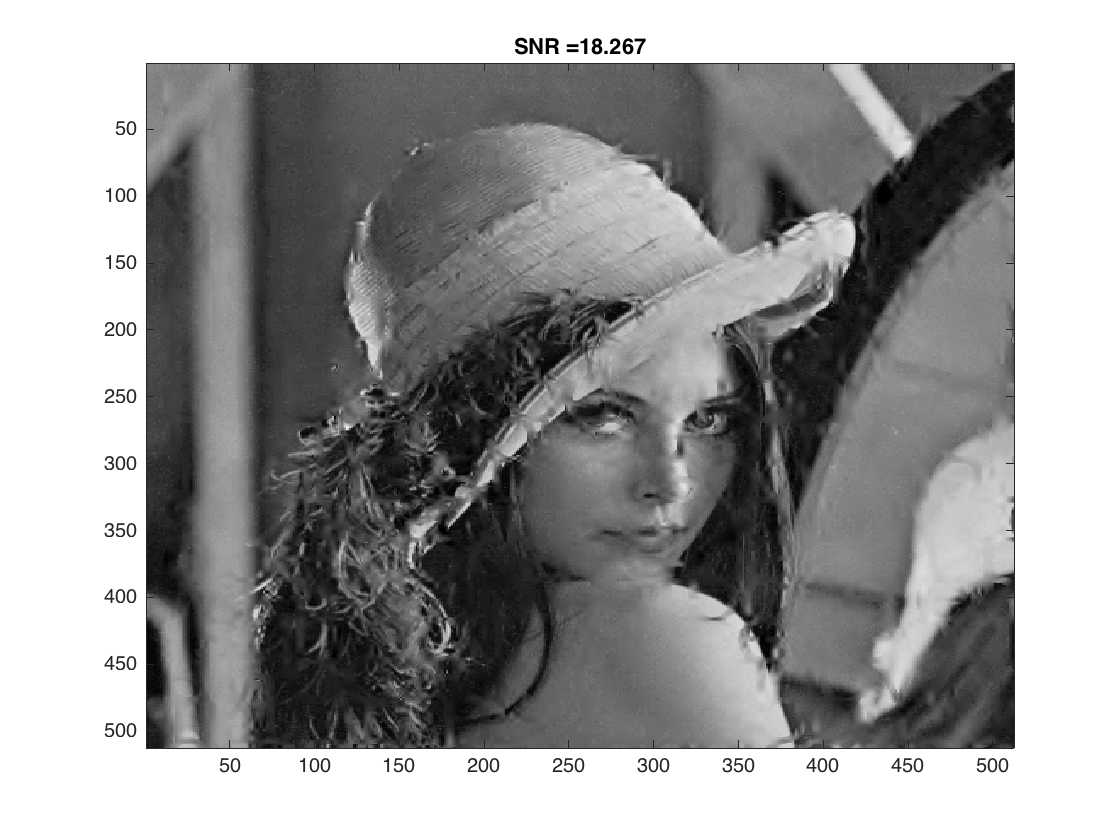
\includegraphics[width=\textwidth]{../src/inpainting/vraag_2_4_db6}
        \caption{\textbf{Daubechies 'db6' wavelet, \\ SNR = $\mathbf{18.26}$} }
        \label{fig:matti_fig_db6}
    \end{subfigure}
    ~ %add desired spacing between images, e. g. ~, \quad, \qquad, \hfill etc. 
    %(or a blank line to force the subfigure onto a new line)
    \begin{subfigure}[b]{0.45\textwidth}
        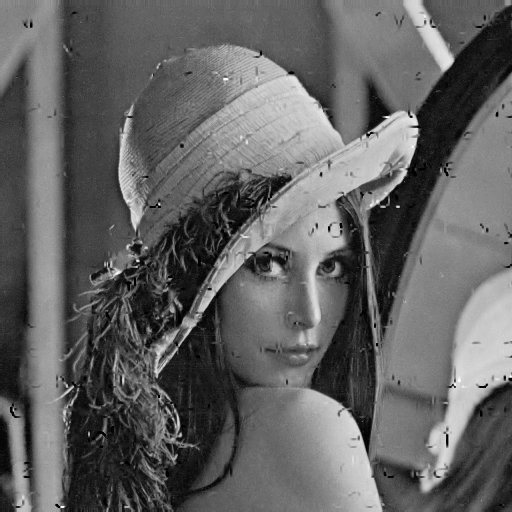
\includegraphics[width=\textwidth]{../src/inpainting/vraag_2_4_bior33}
        \caption{\textbf{ CDF wavelet 'bior3.3', \\ SNR = $\mathbf{11.92}$} }
        \label{fig:matti_fig_bior33}
    \end{subfigure}
        \begin{subfigure}[b]{0.45\textwidth}
        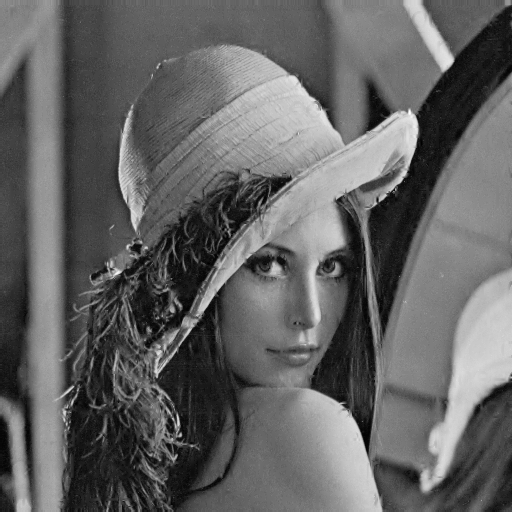
\includegraphics[width=\textwidth]{../src/inpainting/vrag_2_4_coif4}
        \caption{\textbf{ Coiflet wavelet 'coif4', \\ SNR = $\mathbf{18.52}$} }
        \label{fig:matti_fig_coif4}
    \end{subfigure}
    ~ %add desired spacing between images, e. g. ~, \quad, \qquad, \hfill etc. 
    %(or a blank line to force the subfigure onto a new line)
    \begin{subfigure}[b]{0.45\textwidth}
        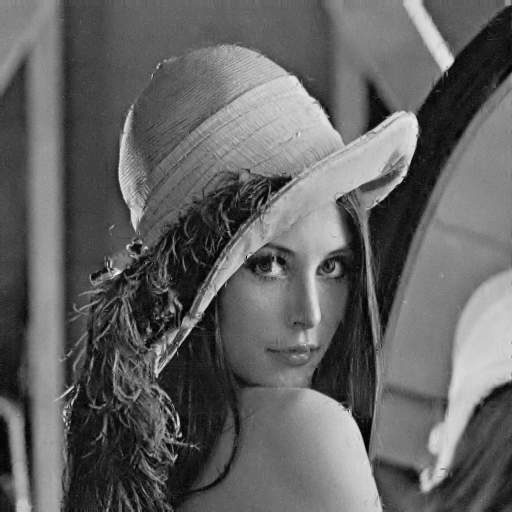
\includegraphics[width=\textwidth]{../src/inpainting/vraag_2_4_sym5}
        \caption{\textbf{ Symlet wavelet 'sym5', \\ SNR = $\mathbf{18.53}$} }
        \label{fig:matti_fig_sym5}
    \end{subfigure}
    \caption{Resultaten van het 'Inpainting' algoritme voor verschillende soorten wavelets. Instellingen algoritme: level $N = 10$, soft thresholding, threshold parameter $\delta = 10$, 200 iteraties.}\label{fig:matti_fig_5}
\end{figure}




